\documentclass{article}

% MISE EN PAGE
\usepackage{pgfplots}
\pgfplotsset{compat=1.18}
\usepackage[margin=2cm]{geometry}
\usepackage{graphicx}
\usepackage{float}
\usepackage{caption}
\usepackage{subcaption}
\usepackage{amsmath}
\usepackage{booktabs}
\usepackage[colorlinks=true, allcolors=black]{hyperref}
\usepackage{balance}
\usepackage{lipsum} % à supprimer une fois que vous mettez votre texte

% TITRE
\title{Artificial Intelligence Insight on Solar Shading}
\author{Amorotti Lucas, Retailleau Mathieu, Aurelian Andrei Panait}
\date{November 2025}

\begin{document}

%%%%%%%%%%%%%%%%%%%%%%%%%%%%%%%%%%%%%%
% PAGE DE GARDE (PLEINE PAGE)
%%%%%%%%%%%%%%%%%%%%%%%%%%%%%%%%%%%%%%
\begin{titlepage}
    \centering

    \vspace*{2cm}

    {\Huge \textbf{Artificial Intelligence–Based Analysis of Solar Shading} \par}
    \vspace{1cm}
    {\Large Amorotti Lucas \\ Retailleau Mathieu \\ Aurelian Andrei Panait\par}
    \vspace{0.5cm}
    {\Large November 2025-February 2026 \par}

    \vfill

    % IMAGE DE LA PAGE DE GARDE (PLEINE LARGEUR)
    \begin{figure}[H]
        \centering
        
\includegraphics[width=\textwidth]{pictures/logo_mines_PSL.png} % votre image ici
    \end{figure}
    \vspace{0.8cm}

{\Large \textbf{Supervised by}}\\[0.2cm]
{\Large Ayoub Hannad}\\
{\Large PhD}

    \vfill

\end{titlepage}

%%%%%%%%%%%%%%%%%%%%%%%%%%%%%%%%%%%%%%
% PAGE 2 : ABSTRACT + TABLE DES MATIÈRES
%%%%%%%%%%%%%%%%%%%%%%%%%%%%%%%%%%%%%%
\clearpage

\begin{abstract}
Predicting building energy consumption traditionally relies on detailed thermal simulations, which are time consuming and require extensive modelling effort. This work evaluates the ability of artificial neural networks to predict energy performance while explicitly considering solar shading effects caused by neighbouring structures. A baseline dataset is generated for a reference building without shading. Additional datasets introduce multiple shading configurations. Two predictive models are trained and assessed using RMSE, CV(RMSE) and R\textsuperscript{2}, and their predictions are compared with dynamic thermal simulations. A renovation scenario is finally tested to quantify whether AI models maintain accuracy when building characteristics are modified. Results demonstrate the influence of shading on prediction accuracy and discuss the capability of machine learning models to integrate physical context.
\end{abstract}

\clearpage
\tableofcontents
\clearpage

%%%%%%%%%%%%%%%%%%%%%%%%%%%%%%%%%%%%%%
% TEXTE EN DEUX COLONNES À PARTIR D'ICI
%%%%%%%%%%%%%%%%%%%%%%%%%%%%%%%%%%%%%%
\twocolumn

\section{Introduction}
The building sector accounts for a significant share of global energy use. Improving its efficiency is essential for reducing environmental impact and achieving climate objectives. Dynamic thermal simulation tools remain the main reference for performance assessment, but they require detailed physical modelling and long computation times. In contrast, machine learning approaches offer faster predictions once trained, provided that the dataset captures the relevant physical behaviour.

Solar shading is one of the parameters that strongly affects energy demand, especially in dense urban environments. Shading modifies solar gains, daylight availability and therefore heating and cooling loads. Despite its impact, shading is often poorly represented in predictive models. This study focuses on analysing how the explicit inclusion of shading parameters affects the performance of neural network models trained to predict building energy consumption.

\section{Methodology}
\subsection{Reference building and simulation dataset}
\subsubsection{Baseline dataset without shading}

\paragraph{Reference building geometry and parameters}

The reference building was modelled using the thermal simulation software \textit{Pléiades}. A four storey building template with nearly identical floors was provided and slightly adapted for this study.

Figures \ref{fig:model3d} and \ref{fig:planrdc} show respectively the 3D external view of the building model and the 2D ground floor plan.

Each floor consists of two rows of five adjacent rooms, each with an individual floor area of 17.04 m$^2$. The two rows are separated by a 1 m wide central corridor. The building is strictly oriented towards the south. Windows are installed on all four façades, ensuring exterior exposure for every room.

\begin{figure}[H]
    \centering
    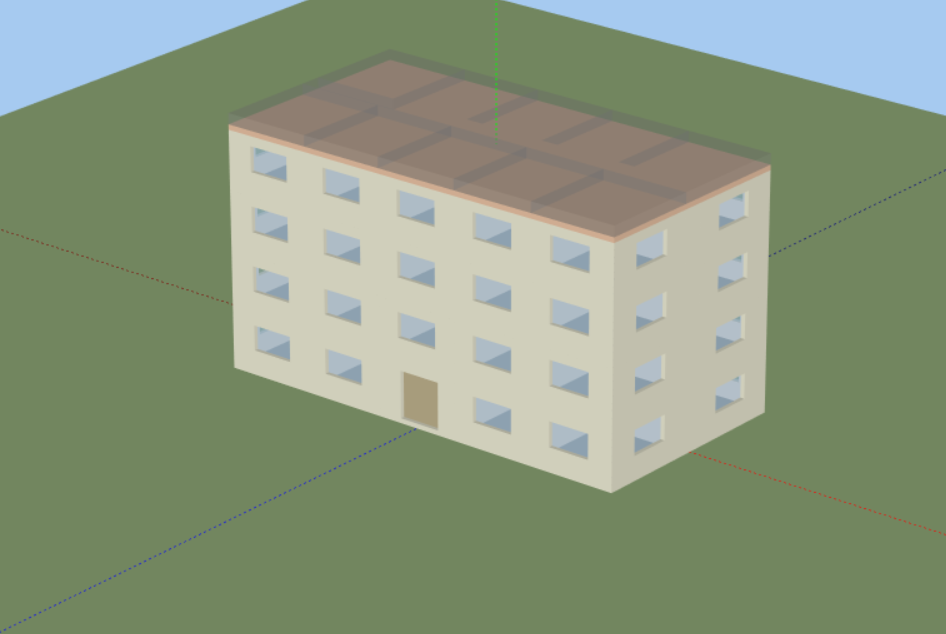
\includegraphics[width=\columnwidth]{pictures/model_de_base.png}
    \caption{3D view of the reference building model}
    \label{fig:model3d}
\end{figure}

\begin{figure}[H]
    \centering
    \includegraphics[width=\columnwidth]{pictures/plan_rdc.png}
    \caption{Ground floor plan of the reference building}
    \label{fig:planrdc}
\end{figure}

\paragraph{Dataset generation process}

To construct the baseline dataset, ten physical and operational variables were randomly sampled within predefined ranges. These variables fall into three categories: ventilation parameters, insulation properties and glazing characteristics.

For each sampled configuration, a full year dynamic thermal simulation was carried out using the AMAPOLA engine integrated in Pléiades.

The dataset was generated in three equally sized subsets:

\begin{itemize}
    \item \textbf{First subset:} parameter values were sampled using a uniform distribution through Latin Hypercube Sampling, ensuring broad coverage of the input space.
    \item \textbf{Second subset:} insulation was set to zero for all simulations, while the remaining variables were sampled normally.
    \item \textbf{Third subset:} insulation was set to zero and ventilation was fixed at its maximum value.
\end{itemize}

Following this procedure, a total of 2000 simulations were obtained. This baseline dataset represents the heating demand of the reference building under conditions where no external shading is present.


\subsubsection{Shading dataset}

\paragraph{Definition of shading scenarios}
To investigate the impact of neighbouring structures on energy needs, a parametric study was conducted involving a single masking obstacle. This obstacle is modelled as a rectangular cuboid with identical dimensions to the reference building ($20 \times 10$ m footprint) and a fixed height $H = 11.5$ m.

The position of the obstacle is defined relative to the reference building using two variables: the azimuth angle and the separation distance $D$.
\begin{itemize}
    \item \textbf{Azimuth:} Five positions are considered relative to the South: $-90^\circ$ (West), $-45^\circ$ (South-West), $0^\circ$ (South), $+45^\circ$ (South-East), and $+90^\circ$ (East).
    \item \textbf{Distance ($D$):} Three wall-to-wall distances are tested: 5 m, 10 m, and 15 m.
\end{itemize}

For the cardinal directions, $D$ represents the perpendicular distance. For the diagonal orientations ($\pm 45^\circ$), a Manhattan distance logic is applied (offset by $D/2$ on both axes).

% FIGURE INTÉGRÉE DANS LA COLONNE (OPTION [H])
\begin{figure}[H]
    \centering
    % Schéma 1 : Positions (Pleine largeur colonne)
    \begin{subfigure}[b]{\columnwidth}
        \centering
        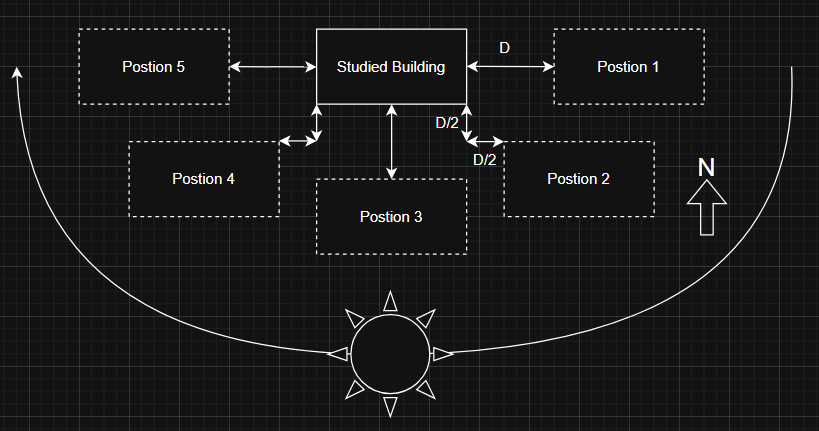
\includegraphics[width=0.95\columnwidth]{pictures/Différentes positions.png}
        \caption{Top-down view of the 5 angular positions}
    \end{subfigure}
    
    \vspace{0.2cm}

    % Schéma 2 : Distances (Pleine largeur colonne)
    \begin{subfigure}[b]{\columnwidth}
        \centering
        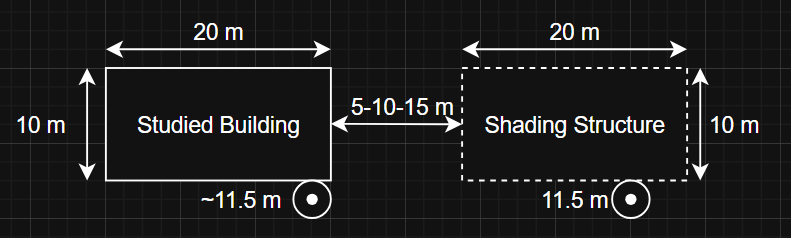
\includegraphics[width=0.95\columnwidth]{pictures/Description batiment.png}
        \caption{Distance definitions ($D$) and geometry}
    \end{subfigure}
    
    \vspace{0.2cm}

    % Rendus 3D (Côte à côte pour gagner de la place)
    \begin{subfigure}[b]{0.48\columnwidth}
        \centering
        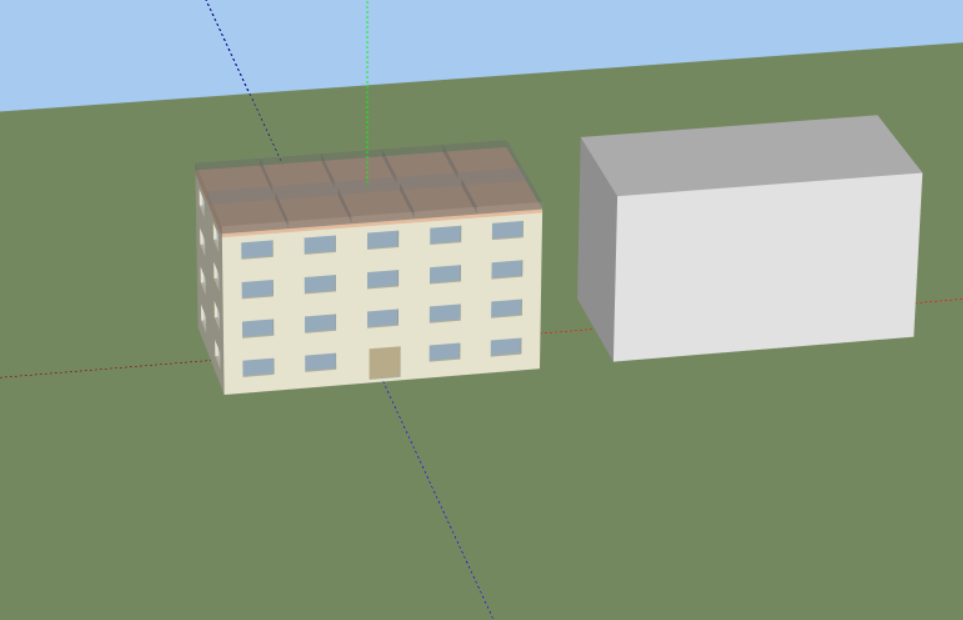
\includegraphics[width=\textwidth]{pictures/1 Est 5m.png}
        \caption{East, $D=5$m}
    \end{subfigure}
    \hfill
    \begin{subfigure}[b]{0.48\columnwidth}
        \centering
        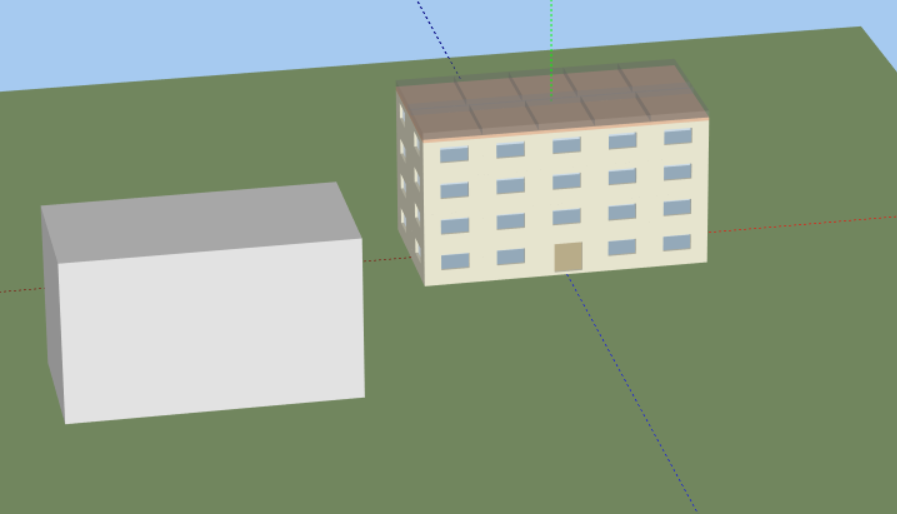
\includegraphics[width=\textwidth]{pictures/14 sud ouest 15m.png}
        \caption{South-West, $D=15$m}
    \end{subfigure}
    
    \caption{Geometric configuration of the shading scenarios. The shading structure ($H=11.5$m) is identical to the reference building.}
    \label{fig:shading_setup}
\end{figure}

This results in a total of 15 distinct shading scenarios ($5 \text{ positions} \times 3 \text{ distances}$).

\paragraph{Dataset expansion strategy}
A specific sampling strategy was employed to isolate the effect of shading from the influence of building envelope parameters. Instead of generating new random building configurations for the shading scenarios, the exact same 2000 building configurations generated for the baseline dataset were reused.

For each of the 15 shading scenarios, the 2000 simulations were re-run with the added obstacle. This "cloning" approach ensures that any variation in energy performance is strictly attributable to the shading effect, as ventilation rates, insulation thicknesses (parameters E2 to E10), and glazing properties (E11, E19) remain strictly identical between the reference and the shaded cases.

Consequently, the total dataset comprises 32,000 simulations:
\begin{itemize}
    \item 2,000 baseline simulations (no shading).
    \item 30,000 shaded simulations (15 scenarios $\times$ 2,000 buildings).
\end{itemize}

The train/test split established in the baseline phase (1600 training / 400 testing) is preserved across all scenarios. The model is trained and tested on the same respective building IDs to prevent data leakage.

\paragraph{Simulation output}
The target variable is the annual heating load [kWh] required to maintain an indoor setpoint temperature of $21^\circ$C. This value is normalized by the total floor area ($754.8 \text{ m}^2$) to obtain kWh/m$^2$. The masks are opaque and oriented at $0^\circ$ (South), significantly impacting direct solar radiation.

\label{sec:mlp-no-shading}


\subsubsection{Renovation scenario}
\paragraph{Envelope and window upgrade measures}

The renovation scenario is introduced as a post-training robustness test. To
keep the analysis consistent with the learning framework, the comparison is
performed strictly through the model inputs. All geometric descriptors and
window-to-wall ratios are kept unchanged, while envelope insulation and glazing
properties are modified to represent an upgraded building.


\begin{table}[H]
\centering
\caption{Renovation scenario: modified model input variables (before / after).}
\label{tab:renovation_inputs}
\scriptsize
\begin{tabular}{lll}
\toprule
Parameters & Before & After \\
\midrule
E2: Internal insulation thickness   & 0.0   & 2.0 \\ \hspace{0.5cm}(external walls)\\
E3: External insulation thickness  & 15.0  & 10.0 \\ \hspace{0.5cm}(external walls)\\
E6: External insulation thickness   & 0.0   & 0.010 \\ \hspace{0.5cm}(staircase walls)\\
E7: Internal insulation thickness   & 0.0   & 2.0 \\ \hspace{0.5cm}(roof)\\
E8: External insulation thickness   & 15.0  & 15.0 \\ \hspace{0.5cm}(roof)\\
E10: Insulation thickness  & 15.0  & 2.0 \\ \hspace{0.5cm}(ground floor)\\
E11: Window thermal conductance  & 2.606 & 1.095 \\ \hspace{0.5cm}(North) \\
E19: Solar factor of glazing   & 0.502 & 0.533 \\ \hspace{0.5cm}(North) \\
E31: Air renewal rate  & 1     & 1 \\ \hspace{0.5cm}(typical floors)\\
E32: Air renewal rate  & 1     & 1 \\ \hspace{0.5cm}(ground floor / corridor)\\
G4: Ground-floor heating enabled  & 1.0   & 1.0 \\
\bottomrule
\end{tabular}
\end{table}


The renovation scenario mainly affects envelope insulation and glazing-related
inputs, while geometric, ventilation and shading parameters remain unchanged.
Internal insulation layers are introduced for external walls and the roof, while
external wall insulation is reduced by approximately 33\%. The most pronounced
change concerns ground floor insulation (E10), which decreases by nearly 87\%.
Window thermal conductance (E11) is reduced by about 58\%, reflecting a
substantial improvement in glazing performance. The solar factor of the glazing
(E19) slightly increases by approximately 6\%, modifying solar gains. Overall,
the renovation induces large relative variations in a limited set of model input
variables, providing a meaningful robustness test for the prediction models.

\begin{figure}[H]
\centering
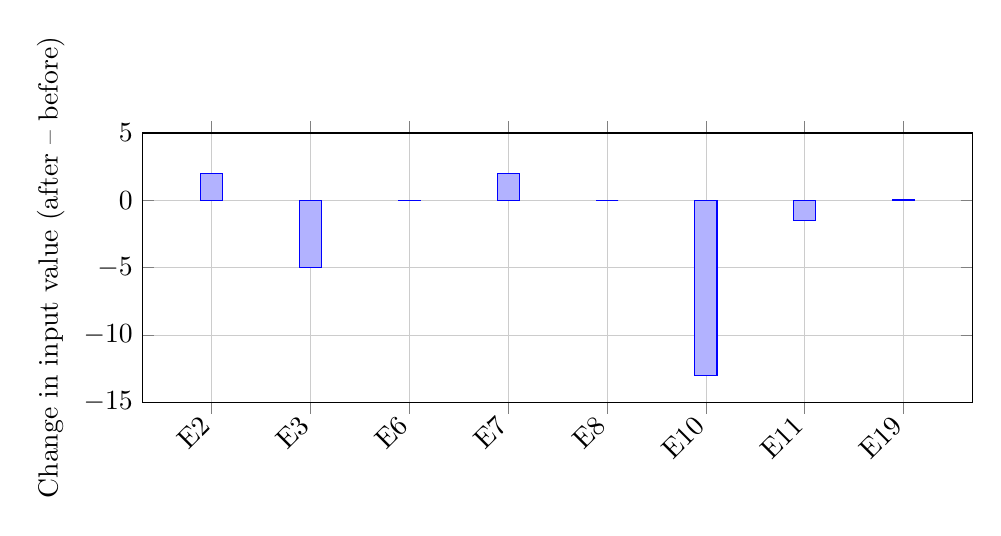
\begin{tikzpicture}
\begin{axis}[
    ybar,
    bar width=8pt,
    height=5.0cm,
    width=\columnwidth,
    ylabel={Change in input value (after -- before)},
    symbolic x coords={E2,E3,E6,E7,E8,E10,E11,E19},
    xtick=data,
    x tick label style={rotate=45, anchor=east},
    ymin=-15, ymax=5,
    grid=both,
    major grid style={line width=.2pt,draw=gray!40},
    minor grid style={line width=.1pt,draw=gray!20},
]
\addplot coordinates {
    (E2,  2.0)
    (E3, -5.0)
    (E6,  0.010)
    (E7,  2.0)
    (E8,  0.0)
    (E10,-13.0)
    (E11,-1.511)
    (E19, 0.031)
};
\end{axis}
\end{tikzpicture}
\label{fig:renovation_deltas}
\end{figure}

\subsection{Preprocessing data}

\subsubsection{Transformation of the data}
Before training the neural network, the raw dataset was preprocessed using 
a unified transformation pipeline. The input variables include numerical, 
categorical and binary descriptors of the building configuration. To ensure 
consistent scaling and a stable learning process, the data were processed 
through a \texttt{ColumnTransformer} composed of four elements:
\begin{itemize}
    \item \textbf{Indicator transformation:} applied to the eight glazing and 
    window-ratio parameters (\textit{Ratio fenêtre Nord, Sud, Est, Ouest} and 
    their corresponding \\ground-floor counterparts). This transformation 
    generates binary or threshold-based indicators that help the model capture 
    abrupt changes in façade configuration.

    \item \textbf{Standardization:} all remaining numerical variables were 
    normalized using a z-score transformation to ensure a balanced contribution 
    during optimization.

    \item \textbf{One-hot encoding:} the categorical variable 
    \textit{Type de mur} was encoded without introducing artificial ordinal 
    relationships.

    \item \textbf{Passthrough:} the binary variable \textit{Chauffage RDC} was 
    preserved unchanged, as no scaling was required.
\end{itemize}


\subsubsection{Training, validation and evaluation metrics}

Each candidate MLP architecture is trained for up to 100 epochs with 
validation-based early stopping. 

After tuning, the best model is evaluated on the test set using the root 
mean squared error (RMSE) and coefficient of determination ($R^2$).

These metrics provide a comprehensive evaluation of model accuracy and 
generalization ability in the no-shading scenario.

\subsection{Network architecture and hyperparameters}

The predictive model is a Multilayer Perceptron (MLP), whose architecture is 
automatically tuned using \texttt{Keras Tuner} via a \texttt{RandomSearch} strategy. 

The hyperparameter search explores:
\begin{itemize}
    \item number of hidden layers: 1 to 10,
    \item neurons per layer: 20 to 500,
    \item activation function: SELU,
    \item kernel initializer: \texttt{lecun\_normal},
    \item learning rate: \(10^{-4}\) to \(3 \cdot 10^{-2}\),
    \item optimizer: stochastic gradient descent with momentum.
\end{itemize}

\section{Results}
% ====== (Preamble) add once if not already present ======
% \usepackage{tikz}
% \usetikzlibrary{positioning}

\subsection{Hyperparameter search summary}

\begin{figure}[H]
\centering

\noindent
\begin{minipage}[t]{0.48\columnwidth}
\centering
\fbox{%
\parbox{0.92\linewidth}{%
\textbf{MLP without shading inputs}\\
\emph{Best configuration \\(random search):}\\[3pt]
\footnotesize
\begin{tabular}{@{}ll@{}}
Hidden layers & \textbf{9} \\
Neurons/layer & \textbf{80} \\
Learning rate & \textbf{0.001} \\
Optimizer     & \textbf{Adam} \\
\end{tabular}
}}
\end{minipage}
\hfill
\begin{minipage}[t]{0.48\columnwidth}
\centering
\fbox{%
\parbox{0.92\linewidth}{%
\textbf{MLP with shading inputs}\\
\emph{Best configuration \\(random search):}\\[3pt]
\footnotesize
\begin{tabular}{@{}ll@{}}
Hidden layers & \textbf{1} \\
Neurons/layer & \textbf{20} \\
Learning rate & \textbf{0.01} \\
Optimizer     & \textbf{Adam} \\
\end{tabular}
}}
\end{minipage}

\caption{Best hyperparameter configurations selected by random search for the two
input scenarios. The shading-aware optimum is reported; the no-shading optimum
will be added once the tuning run completes.}
\label{fig:hp_cards}
\end{figure}


The random hyperparameter search yields a compact configuration for the shading-aware
model, consisting of a single hidden layer with 20 neurons, trained with the Adam
optimizer and a learning rate of 0.01. This outcome suggests that, once shading
information is explicitly provided at the input level, the mapping from inputs to
annual heating demand can be captured with limited model complexity. The same search
procedure is applied to the no-shading case; its best configuration will be reported
once the tuning run is completed, enabling a direct comparison of how the optimal
capacity depends on the chosen input space.

\subsection{Models performance}

This section compares the predictive performance of the two proposed models:
(i) a baseline MLP trained without shading-related inputs, and (ii) a
shading-aware MLP explicitly incorporating geometric shading parameters. Model
performance is assessed using graphical indicators and standard regression
metrics computed on an independent test set.

\subsubsection{Baseline model (without shading inputs)}

The baseline model is first evaluated to establish a reference level of
performance. Figure~\ref{fig:scatter_baseline} compares predicted and simulated
annual heating demand on the test dataset.

Predictions are generally well aligned with the identity line, indicating a
strong overall agreement between model outputs and simulation results.
Nevertheless, a slight increase in dispersion can be observed for certain
configurations, particularly those associated with strong solar masking.
Because shading information is not explicitly provided as an input, the model
must implicitly infer these effects from the remaining variables, which may
limit its robustness in highly shaded situations.

\begin{figure}[H]
\centering
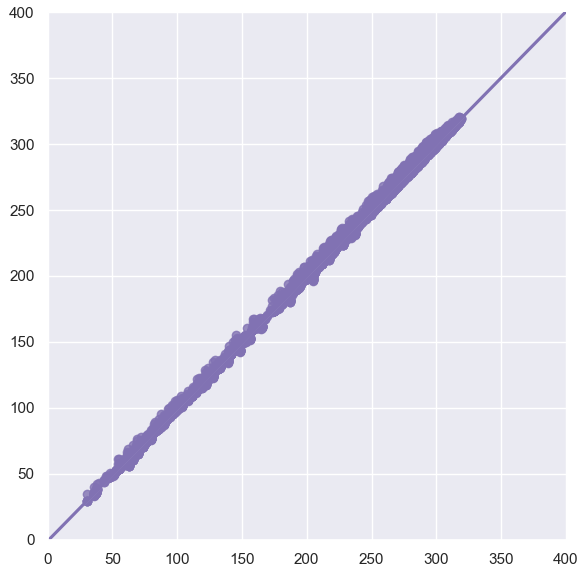
\includegraphics[width=\columnwidth]{pictures/scatter_baseline.png}
\caption{Predicted versus simulated heating demand for the baseline model. The
solid line represents the identity line.}
\label{fig:scatter_baseline}
\end{figure}

\subsubsection{Shading-aware model}

The shading-aware model is evaluated using the same test dataset and performance
metrics as the baseline model. Figure~\ref{fig:scatter_shading} presents the
comparison between predicted and simulated heating demand.

Compared to the baseline configuration, predictions remain more tightly
distributed around the identity line across the full range of values. This
reduced dispersion indicates that the explicit inclusion of shading-related
inputs improves the model’s ability to capture variations in solar gains induced
by neighbouring obstacles, resulting in a more consistent prediction behaviour.

\begin{figure}[H]
\centering
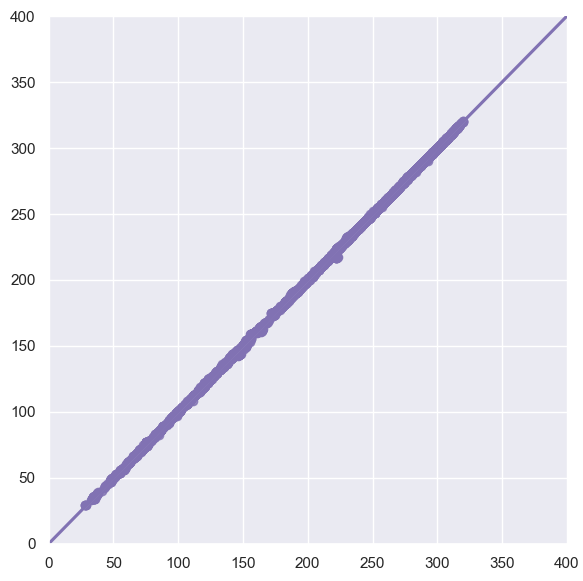
\includegraphics[width=\columnwidth]{pictures/scatter_shading.png}
\caption{Predicted versus simulated heating demand for the shading-aware model.}
\label{fig:scatter_shading}
\end{figure}

\subsubsection{Quantitative performance metrics}

Quantitative performance indicators are summarized in
Table~\ref{tab:model_metrics}. Both models achieve high predictive accuracy on
the test set, as reflected by very high coefficients of determination.

\begin{table}[H]
\centering
\caption{Prediction performance of both models on the test dataset.}
\label{tab:model_metrics}
\scriptsize
\begin{tabular}{lccc}
\toprule
Model & RMSE & CV(RMSE) [\%] & $R^2$ \\
\midrule
MLP without shading & 2.1047 & 0.96\% & 0.9991 \\

MLP with shading & 0.5977 & 0.27\% & 0.9999 \\
\bottomrule
\end{tabular}
\end{table}


However, the shading-aware model systematically outperforms the baseline model,
with a reduction of approximately 72\% in RMSE and a CV(RMSE) below 0.3\%.
These results confirm that incorporating shading information leads not only to
slightly improved accuracy but also to a more stable and robust prediction
across different operating conditions.

Both models achieve high predictive accuracy on the test set. However, the
shading-aware model consistently exhibits lower error levels and a more stable
coefficient of determination, particularly for configurations where shading
significantly affects heating demand.

\subsubsection{Impact of shading scenarios}

Several important trends can be observed. 

\begin{figure}[H]
\centering
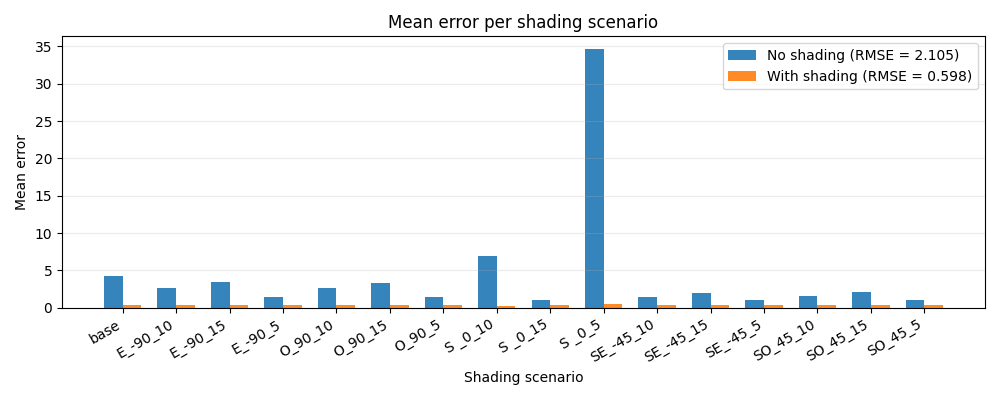
\includegraphics[width=\columnwidth]{pictures/hist_shading.png}
\caption{Prediction error distribution across shading scenarios for both models.}
\label{fig:error_shading}
\end{figure}


First, the baseline model
exhibits a strong sensitivity to the shading configuration, with error levels
varying significantly across scenarios. In particular, configurations involving
southern orientations at short distances lead to a sharp increase in prediction
error, reaching values several times higher than in weakly shaded cases. This
behaviour highlights the inability of the baseline model to correctly account
for strong solar masking effects when shading information is not explicitly
provided.

In contrast, the shading-aware model exhibits a much more stable error
distribution across all scenarios. The mean error remains low and relatively
uniform, regardless of obstacle orientation or distance. This confirms that the
introduction of shading-related inputs allows the model to capture the impact of
solar obstruction in a consistent manner, significantly reducing sensitivity to
specific geometric configurations.

The comparison also reveals that the performance gap between the two models
increases as shading becomes more pronounced. While both models perform
similarly in weakly shaded cases, the baseline model rapidly degrades under
strong shading conditions, whereas the shading-aware model maintains a low and
nearly constant error level. This result highlights the key role of shading
information in improving robustness and confirms that solar masking constitutes
a major source of prediction error when not explicitly accounted for.

Overall, these results demonstrate that incorporating shading parameters does
not only reduce the global prediction error, but also ensures a more uniform and
physically consistent behavior across diverse shading configurations.


\subsubsection{Model interpretability}

To improve model interpretability, SHAP values are computed for the
shading-aware model. Figure~\ref{fig:shap_summary} presents a global summary of
feature contributions to the predicted heating demand.

Envelope insulation thicknesses and glazing-related parameters are identified as
the dominant contributors, in agreement with physical expectations. Shading
descriptors also exhibit a significant contribution, with their impact varying
across configurations. The dispersion of SHAP values highlights the nonlinear
interaction between shading, envelope properties and heating demand, confirming
that geometric context plays a meaningful role in the model’s predictions.


\begin{figure}[H]
\centering
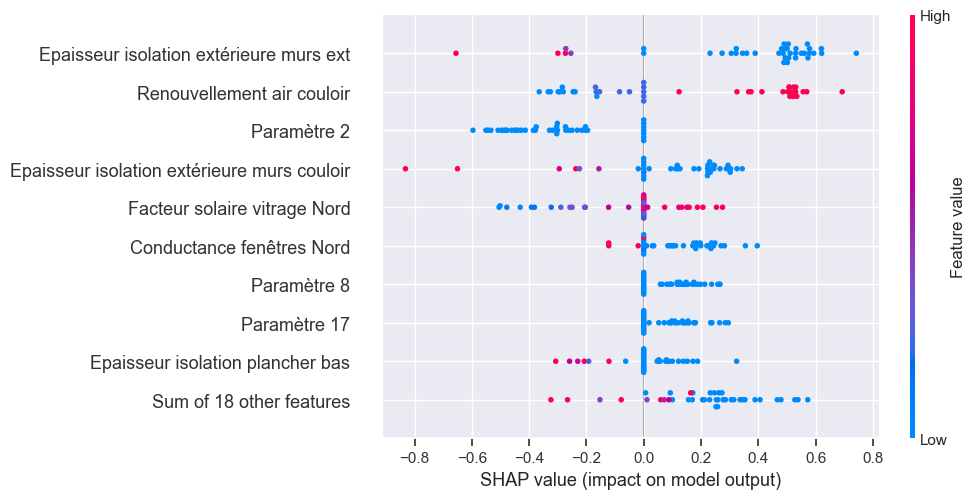
\includegraphics[width=\columnwidth]{pictures/shap_summary.png}
\caption{SHAP summary plot for the shading-aware model.}
\label{fig:shap_summary}
\end{figure}
\subsubsection{Performance under renovation conditions}

\begin{table}[H]
\centering
\caption{Model performance before and after renovation.}
\label{tab:renovation_performance}
\scriptsize
\begin{tabular}{lcc}
\toprule
Model & Consumption ($kWh/m^2$) (before) & Consumption ($kWh/m^2$) (after) \\
\midrule
MLP without shading & 108.59131 &  109.77188\\
MLP with shading    & 106.23883 & 104.5243 \\
\bottomrule
\end{tabular}
\end{table}

Finally, both models are evaluated under the renovation scenario to assess their
robustness to changes in envelope and glazing characteristics.
Table~\ref{tab:renovation_performance} compares prediction errors before and
after renovation.

While both models experience changes in prediction accuracy following
renovation, the shading-aware model maintains a more stable performance level.
This behaviour suggests a better generalization capability when the input space
is modified, supporting the relevance of explicitly incorporating shading
information even when building characteristics differ from those seen during
training.
It should be noted that, unlike the results reported in Table 2 (expressed in kWh/m²), the renovation scenario errors presented in Table 3 are reported in absolute kWh. This difference in normalization explains the significantly higher RMSE values observed after renovation.

\section{Discussion}
\subsection{Influence of shading on learning and prediction}
The results clearly demonstrate that solar shading has a significant influence on the learning process and predictive accuracy of neural network models for building energy demand, as evidenced by the strong reduction in prediction error obtained when shading-related inputs are introduced (Table~\ref{tab:model_metrics}). When shading information is not explicitly included, the baseline model is forced to implicitly infer solar masking effects from unrelated envelope and operational variables, since the input space does not contain any geometric descriptors of
neighbouring obstacles (Section~2.1.2). This limitation leads to increased dispersion in predictions, particularly for configurations with strong or asymmetric shading, as observed in the predicted versus simulated results for the baseline model (Figure~\ref{fig:scatter_baseline}).
In contrast, the shading-aware model benefits from a more physically informed input space. By explicitly encoding geometric shading descriptors such as obstacle azimuth and separation distance (Section~2.1.2), the model is able to directly associate variations in solar gains with changes in heating demand. This results in a substantial reduction in prediction error (Table~\ref{tab:model_metrics}) and a more stable regression behaviour across shading configurations, as illustrated by the tighter alignment with the identity line (Figure~\ref{fig:scatter_shading}) and the more uniform error distribution across shading scenarios (Figure~\ref{fig:error_shading}). The marked improvement in RMSE and CV(RMSE) confirms that shading is not a secondary effect but a key driver of model performance when predicting energy demand in dense or obstructed environments.
\subsection{Strengths and limitations of the proposed approach}
One of the main strengths of the proposed approach lies in the controlled
construction of the simulation dataset. By reusing identical building
configurations across all shading scenarios, the study isolates the impact of
solar shading from other envelope and operational parameters
(Section~2.1.2). This design ensures that observed differences in predictive
performance can be directly attributed to shading effects rather than to
confounding variability in the input space.

Another key strength is the integration of physically meaningful descriptors
into a data-driven modelling framework. The inclusion of geometric shading
parameters enables the model to learn relationships that are consistent with
building physics, as reflected by the improved prediction accuracy and reduced
dispersion observed for the shading-aware model
(Figures~\ref{fig:scatter_shading} and~\ref{fig:scatter_baseline}). The SHAP
analysis further supports this interpretation by highlighting the contribution
of shading-related features alongside envelope and glazing parameters
(Figure~\ref{fig:shap_summary}).

Despite these advantages, several limitations should be acknowledged. The
shading configurations considered in this study are deliberately simplified,
involving a single neighbouring obstacle with fixed height and idealized
geometry. Real urban environments typically include multiple surrounding
buildings with varying shapes, heights and surface properties, which may lead
to more complex shading interactions than those captured here.

In addition, the models are trained exclusively on simulation-generated data.
While this ensures consistency and physical coherence, it may limit direct
transferability to real-world buildings, where uncertainties related to
construction quality, occupant behaviour and weather variability are more
pronounced. Finally, although the shading-aware model demonstrates strong
predictive performance within the explored parameter space, extrapolation
beyond the training ranges cannot be guaranteed and should be approached with
caution.
\subsection{Applicability for early design and renovation analysis}
The proposed modelling framework is particularly relevant for early-stage design
and renovation analysis, where rapid evaluation of multiple configurations is
required while detailed information about building components may still be
limited. At these stages, full dynamic thermal simulations remain time-consuming
and computationally expensive, making them less suitable for iterative
exploration of design alternatives.

Once trained, the neural network models provide near-instantaneous predictions
of annual heating demand while preserving sensitivity to key physical drivers,
including envelope properties and solar shading effects. The strong agreement
between predicted and simulated values observed for the shading-aware model
(Figure~\ref{fig:scatter_shading}) indicates that the approach can reliably
approximate simulation results at a fraction of the computational cost.

The renovation scenario further illustrates the applicability of the method in
decision-support contexts. Despite significant modifications to insulation and
glazing parameters (Table~\ref{tab:renovation_inputs}), the shading-aware model
maintains a stable level of predictive accuracy after renovation
(Table~\ref{tab:renovation_performance}). This robustness suggests that the model
captures generalizable relationships between inputs and energy demand, rather
than overfitting to a narrow range of building configurations.

As a result, the proposed approach can be effectively used as a screening or
preliminary assessment tool to compare design and renovation options, identify
the relative importance of shading effects, and prioritize configurations for
more detailed simulation-based analysis. Such a workflow is particularly
valuable in dense urban contexts, where solar masking plays a critical role in
building energy performance.
\subsection{Sources of error and possible improvements}

In the proposed approach, shading effects are introduced through a finite number
of predefined configurations. While this strategy allows a controlled analysis
of the impact of shading, it also implies that solar obstruction is represented
in a discrete manner. In practice, it is not possible to enumerate all possible
shading configurations, as real urban environments exhibit a continuous range of
geometric situations resulting from building positions, heights, orientations
and mutual interactions.

This discretization limits the capacity of the model to generalize beyond the
simulated cases. Although the neural network learns the influence of shading for
the considered configurations, it cannot directly infer the effect of
intermediate or unseen situations. As a consequence, the model remains
case-dependent and its applicability to arbitrary urban layouts is inherently
restricted.

Moreover, shading is intrinsically a time-dependent phenomenon. Its impact
varies continuously throughout the day and over the year as a function of solar
altitude and azimuth. By encoding shading only through static scenario labels,
the model does not receive explicit information about when shading occurs, how
long it lasts, or how it evolves over time. Even though this temporal variability
is implicitly present in the simulation outputs, it is not explicitly available
in the input space, which prevents the model from learning fine-grained
solar–thermal interactions.

This limitation suggests that a more general and physically consistent approach
would rely on continuous shading descriptors rather than discrete cases. Such
descriptors could include geometric parameters (e.g. obstacle orientation,
distance, height ratios) or radiative indicators derived from sun-path analysis,
such as shadow duration or solar obstruction factors. Introducing these features
would enable the model to capture the temporal dynamics of shading and to
generalize more effectively to complex and realistic urban configurations.


\section{Conclusion}
\subsection{Key findings}
This study demonstrates that explicitly incorporating solar shading information
into data-driven building energy models significantly improves predictive
accuracy. Compared to a baseline neural network trained without shading-related
inputs, the shading-aware model achieves a substantial reduction in prediction
error, with RMSE decreased by approximately 72\% and CV(RMSE) below 0.3.

The results further show that neglecting shading forces baseline models to
implicitly infer solar masking effects from unrelated envelope and operational
variables, leading to increased dispersion in predictions for highly shaded
configurations. In contrast, the inclusion of geometric shading descriptors
enables the model to directly capture variations in solar gains induced by
neighbouring obstacles, resulting in more consistent prediction behaviour across
different shading scenarios.

Finally, the robustness analysis under renovation conditions indicates that the
shading-aware model maintains stable performance when building envelope and
glazing properties are modified. This suggests that the proposed approach learns
generalizable relationships between physical inputs and energy demand, supporting
its potential use as a fast and reliable decision-support tool in early design
and renovation contexts.
\subsection{Role of shading in predictive energy modelling}
The results of this study highlight the central role of solar shading as a
structuring variable in predictive energy modelling. Rather than acting as a
secondary correction, shading directly influences solar gains and therefore
constitutes a key driver of heating demand, particularly in dense or obstructed
urban environments.

From a modelling perspective, the explicit inclusion of shading-related
descriptors allows data-driven approaches to better reflect the underlying
physical mechanisms governing building energy performance. When shading is not
represented in the input space, predictive models are forced to approximate its
effects indirectly through envelope or operational parameters, which can reduce
robustness and increase prediction dispersion. By contrast, shading-aware input
spaces enable a clearer mapping between geometry, solar exposure and energy
demand.

These findings suggest that future predictive energy models, especially those
intended for urban-scale applications or early-stage design support, should
systematically integrate shading information alongside conventional envelope
and system parameters. Doing so improves not only predictive accuracy but also
model interpretability and physical consistency, reinforcing the relevance of
hybrid approaches that combine geometric context with machine learning methods.
\subsection{Future work}
Several directions can be explored to extend the scope and applicability of the
proposed approach. First, the representation of shading could be refined by
considering more complex urban configurations, including multiple neighbouring
obstacles with varying heights, shapes and spatial arrangements. Such extensions
would allow the model to better capture the diversity and geometric complexity of
real-world urban environments, in line with recent developments in urban
building energy modelling (UBEM) \cite{Ferrando2021UBEM,Ali2021UBEM}.

Future work could also investigate the generalization of the proposed models
across different climatic conditions and building typologies. Training and
evaluating the framework on datasets generated for multiple climates, or
validating predictions against measured building energy consumption, would
provide valuable insight into model robustness and transferability beyond the
controlled simulation context.

From a methodological perspective, the integration of hybrid modelling strategies
represents a promising avenue. In particular, combining data-driven approaches
with simplified physical constraints or physics-informed neural networks (PINNs)
could improve extrapolation capabilities while preserving computational
efficiency \cite{Raissi2019PINNs,Karniadakis2021PIML}. Finally, extending the
framework to include cooling demand and multi-objective performance indicators
would further enhance its relevance for early-stage design and renovation
decision support.

\bibliographystyle{unsrt}
\bibliography{references}
\end{document}
